\documentclass[1p]{elsarticle_modified}
%\bibliographystyle{elsarticle-num}

%\usepackage[colorlinks]{hyperref}
%\usepackage{abbrmath_seonhwa} %\Abb, \Ascr, \Acal ,\Abf, \Afrak
\usepackage{amsfonts}
\usepackage{amssymb}
\usepackage{amsmath}
\usepackage{amsthm}
\usepackage{scalefnt}
\usepackage{amsbsy}
\usepackage{kotex}
\usepackage{caption}
\usepackage{subfig}
\usepackage{color}
\usepackage{graphicx}
\usepackage{xcolor} %% white, black, red, green, blue, cyan, magenta, yellow
\usepackage{float}
\usepackage{setspace}
\usepackage{hyperref}

\usepackage{tikz}
\usetikzlibrary{arrows}

\usepackage{multirow}
\usepackage{array} % fixed length table
\usepackage{hhline}

%%%%%%%%%%%%%%%%%%%%%
\makeatletter
\renewcommand*\env@matrix[1][\arraystretch]{%
	\edef\arraystretch{#1}%
	\hskip -\arraycolsep
	\let\@ifnextchar\new@ifnextchar
	\array{*\c@MaxMatrixCols c}}
\makeatother %https://tex.stackexchange.com/questions/14071/how-can-i-increase-the-line-spacing-in-a-matrix
%%%%%%%%%%%%%%%

\usepackage[normalem]{ulem}

\newcommand{\msout}[1]{\ifmmode\text{\sout{\ensuremath{#1}}}\else\sout{#1}\fi}
%SOURCE: \msout is \stkout macro in https://tex.stackexchange.com/questions/20609/strikeout-in-math-mode

\newcommand{\cancel}[1]{
	\ifmmode
	{\color{red}\msout{#1}}
	\else
	{\color{red}\sout{#1}}
	\fi
}

\newcommand{\add}[1]{
	{\color{blue}\uwave{#1}}
}

\newcommand{\replace}[2]{
	\ifmmode
	{\color{red}\msout{#1}}{\color{blue}\uwave{#2}}
	\else
	{\color{red}\sout{#1}}{\color{blue}\uwave{#2}}
	\fi
}

\newcommand{\Sol}{\mathcal{S}} %segment
\newcommand{\D}{D} %diagram
\newcommand{\A}{\mathcal{A}} %arc


%%%%%%%%%%%%%%%%%%%%%%%%%%%%%5 test

\def\sl{\operatorname{\textup{SL}}(2,\Cbb)}
\def\psl{\operatorname{\textup{PSL}}(2,\Cbb)}
\def\quan{\mkern 1mu \triangleright \mkern 1mu}

\theoremstyle{definition}
\newtheorem{thm}{Theorem}[section]
\newtheorem{prop}[thm]{Proposition}
\newtheorem{lem}[thm]{Lemma}
\newtheorem{ques}[thm]{Question}
\newtheorem{cor}[thm]{Corollary}
\newtheorem{defn}[thm]{Definition}
\newtheorem{exam}[thm]{Example}
\newtheorem{rmk}[thm]{Remark}
\newtheorem{alg}[thm]{Algorithm}

\newcommand{\I}{\sqrt{-1}}
\begin{document}

%\begin{frontmatter}
%
%\title{Boundary parabolic representations of knots up to 8 crossings}
%
%%% Group authors per affiliation:
%\author{Yunhi Cho} 
%\address{Department of Mathematics, University of Seoul, Seoul, Korea}
%\ead{yhcho@uos.ac.kr}
%
%
%\author{Seonhwa Kim} %\fnref{s_kim}}
%\address{Center for Geometry and Physics, Institute for Basic Science, Pohang, 37673, Korea}
%\ead{ryeona17@ibs.re.kr}
%
%\author{Hyuk Kim}
%\address{Department of Mathematical Sciences, Seoul National University, Seoul 08826, Korea}
%\ead{hyukkim@snu.ac.kr}
%
%\author{Seokbeom Yoon}
%\address{Department of Mathematical Sciences, Seoul National University, Seoul, 08826,  Korea}
%\ead{sbyoon15@snu.ac.kr}
%
%\begin{abstract}
%We find all boundary parabolic representation of knots up to 8 crossings.
%
%\end{abstract}
%\begin{keyword}
%    \MSC[2010] 57M25 
%\end{keyword}
%
%\end{frontmatter}

%\linenumbers
%\tableofcontents
%
\newcommand\colored[1]{\textcolor{white}{\rule[-0.35ex]{0.8em}{1.4ex}}\kern-0.8em\color{red} #1}%
%\newcommand\colored[1]{\textcolor{white}{ #1}\kern-2.17ex	\textcolor{white}{ #1}\kern-1.81ex	\textcolor{white}{ #1}\kern-2.15ex\color{red}#1	}

{\Large $\underline{12a_{0665}~(K12a_{0665})}$}

\setlength{\tabcolsep}{10pt}
\renewcommand{\arraystretch}{1.6}
\vspace{1cm}\begin{tabular}{m{100pt}>{\centering\arraybackslash}m{274pt}}
\multirow{5}{120pt}{
	\centering
	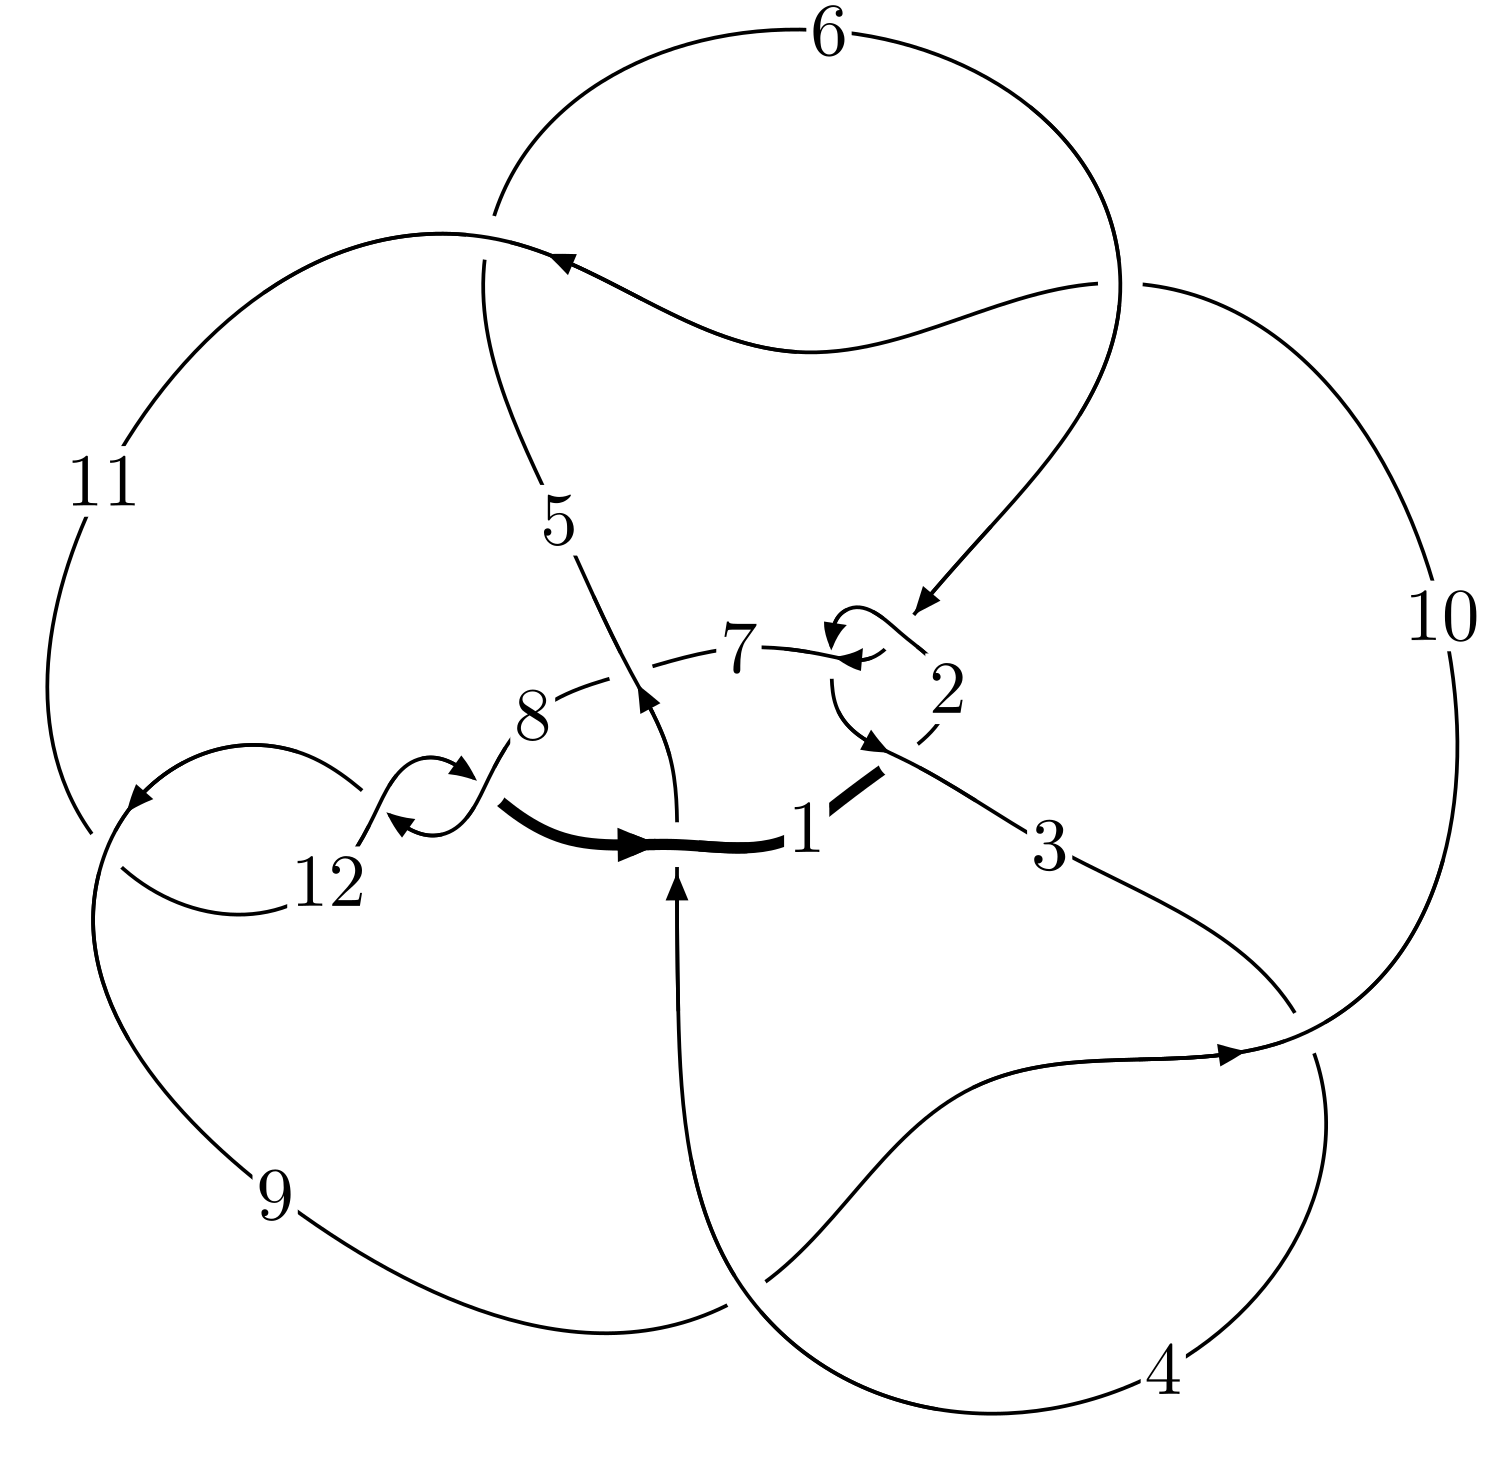
\includegraphics[width=112pt]{../../../GIT/diagram.site/Diagrams/png/1466_12a_0665.png}\\
\ \ \ A knot diagram\footnotemark}&
\allowdisplaybreaks
\textbf{Linearized knot diagam} \\
\cline{2-2}
 &
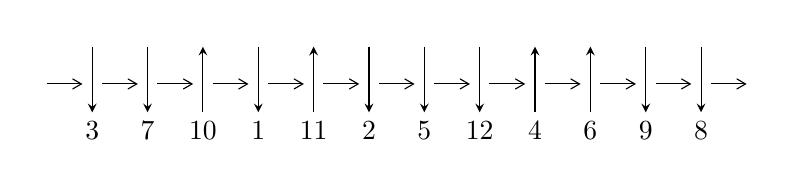
\begin{tikzpicture}[x=20pt, y=17pt]
	% nodes
	\node (C0) at (0, 0) {};
	\node (C1) at (1, 0) {};
	\node (C1U) at (1, +1) {};
	\node (C1D) at (1, -1) {3};

	\node (C2) at (2, 0) {};
	\node (C2U) at (2, +1) {};
	\node (C2D) at (2, -1) {7};

	\node (C3) at (3, 0) {};
	\node (C3U) at (3, +1) {};
	\node (C3D) at (3, -1) {10};

	\node (C4) at (4, 0) {};
	\node (C4U) at (4, +1) {};
	\node (C4D) at (4, -1) {1};

	\node (C5) at (5, 0) {};
	\node (C5U) at (5, +1) {};
	\node (C5D) at (5, -1) {11};

	\node (C6) at (6, 0) {};
	\node (C6U) at (6, +1) {};
	\node (C6D) at (6, -1) {2};

	\node (C7) at (7, 0) {};
	\node (C7U) at (7, +1) {};
	\node (C7D) at (7, -1) {5};

	\node (C8) at (8, 0) {};
	\node (C8U) at (8, +1) {};
	\node (C8D) at (8, -1) {12};

	\node (C9) at (9, 0) {};
	\node (C9U) at (9, +1) {};
	\node (C9D) at (9, -1) {4};

	\node (C10) at (10, 0) {};
	\node (C10U) at (10, +1) {};
	\node (C10D) at (10, -1) {6};

	\node (C11) at (11, 0) {};
	\node (C11U) at (11, +1) {};
	\node (C11D) at (11, -1) {9};

	\node (C12) at (12, 0) {};
	\node (C12U) at (12, +1) {};
	\node (C12D) at (12, -1) {8};
	\node (C13) at (13, 0) {};

	% arrows
	\draw[->,>={angle 60}]
	(C0) edge (C1) (C1) edge (C2) (C2) edge (C3) (C3) edge (C4) (C4) edge (C5) (C5) edge (C6) (C6) edge (C7) (C7) edge (C8) (C8) edge (C9) (C9) edge (C10) (C10) edge (C11) (C11) edge (C12) (C12) edge (C13) ;	\draw[->,>=stealth]
	(C1U) edge (C1D) (C2U) edge (C2D) (C3D) edge (C3U) (C4U) edge (C4D) (C5D) edge (C5U) (C6U) edge (C6D) (C7U) edge (C7D) (C8U) edge (C8D) (C9D) edge (C9U) (C10D) edge (C10U) (C11U) edge (C11D) (C12U) edge (C12D) ;
	\end{tikzpicture} \\
\hhline{~~} \\& 
\textbf{Solving Sequence} \\ \cline{2-2} 
 &
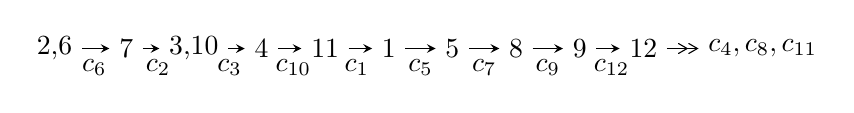
\begin{tikzpicture}[x=23pt, y=7pt]
	% node
	\node (A0) at (-1/8, 0) {2,6};
	\node (A1) at (1, 0) {7};
	\node (A2) at (33/16, 0) {3,10};
	\node (A3) at (25/8, 0) {4};
	\node (A4) at (33/8, 0) {11};
	\node (A5) at (41/8, 0) {1};
	\node (A6) at (49/8, 0) {5};
	\node (A7) at (57/8, 0) {8};
	\node (A8) at (65/8, 0) {9};
	\node (A9) at (73/8, 0) {12};
	\node (C1) at (1/2, -1) {$c_{6}$};
	\node (C2) at (3/2, -1) {$c_{2}$};
	\node (C3) at (21/8, -1) {$c_{3}$};
	\node (C4) at (29/8, -1) {$c_{10}$};
	\node (C5) at (37/8, -1) {$c_{1}$};
	\node (C6) at (45/8, -1) {$c_{5}$};
	\node (C7) at (53/8, -1) {$c_{7}$};
	\node (C8) at (61/8, -1) {$c_{9}$};
	\node (C9) at (69/8, -1) {$c_{12}$};
	\node (A10) at (11, 0) {$c_{4},c_{8},c_{11}$};

	% edge
	\draw[->,>=stealth]	
	(A0) edge (A1) (A1) edge (A2) (A2) edge (A3) (A3) edge (A4) (A4) edge (A5) (A5) edge (A6) (A6) edge (A7) (A7) edge (A8) (A8) edge (A9) ;
	\draw[->>,>={angle 60}]	
	(A9) edge (A10);
\end{tikzpicture} \\ 

\end{tabular} \\

\footnotetext{
The image of knot diagram is generated by the software ``\textbf{Draw programme}" developed by Andrew Bartholomew(\url{http://www.layer8.co.uk/maths/draw/index.htm\#Running-draw}), where we modified some parts for our purpose(\url{https://github.com/CATsTAILs/LinksPainter}).
}\phantom \\ \newline 
\centering \textbf{Ideals for irreducible components\footnotemark of $X_{\text{par}}$} 
 
\begin{align*}
I^u_{1}&=\langle 
3349 u^{42}-43719 u^{41}+\cdots+64 b+14656,\;-3589 u^{42}+50017 u^{41}+\cdots+128 a-81280,\\
\phantom{I^u_{1}}&\phantom{= \langle  }u^{43}-15 u^{42}+\cdots-1216 u+128\rangle \\
I^u_{2}&=\langle 
-4164019282 a^5 u^5-75372960680 u^5 a^4+\cdots-521321653767 a-34419126350,\\
\phantom{I^u_{2}}&\phantom{= \langle  }- u^5 a^4-3 u^5 a^3+\cdots+3 a+4,\;u^6+u^5- u^4-2 u^3+u+1\rangle \\
I^u_{3}&=\langle 
2.29399\times10^{20} a^{7} u^{5}-2.53388\times10^{20} a^{6} u^{5}+\cdots-6.52305\times10^{21} a-2.07651\times10^{21},\\
\phantom{I^u_{3}}&\phantom{= \langle  }- a^7 u^5-3 a^6 u^5+\cdots-26 a^2-4 a,\;u^6+u^5- u^4-2 u^3+u+1\rangle \\
I^u_{4}&=\langle 
u^{29}+6 u^{28}+\cdots+b-21,\;25 u^{29}-4 u^{28}+\cdots+2 a+57,\;u^{30}-9 u^{28}+\cdots+5 u+2\rangle \\
\\
\end{align*}
\raggedright * 4 irreducible components of $\dim_{\mathbb{C}}=0$, with total 157 representations.\\
\footnotetext{All coefficients of polynomials are rational numbers. But the coefficients are sometimes approximated in decimal forms when there is not enough margin.}
\newpage
\renewcommand{\arraystretch}{1}
\centering \section*{I. $I^u_{1}= \langle 3349 u^{42}-43719 u^{41}+\cdots+64 b+14656,\;-3589 u^{42}+50017 u^{41}+\cdots+128 a-81280,\;u^{43}-15 u^{42}+\cdots-1216 u+128 \rangle$}
\flushleft \textbf{(i) Arc colorings}\\
\begin{tabular}{m{7pt} m{180pt} m{7pt} m{180pt} }
\flushright $a_{2}=$&$\begin{pmatrix}0\\u\end{pmatrix}$ \\
\flushright $a_{6}=$&$\begin{pmatrix}1\\0\end{pmatrix}$ \\
\flushright $a_{7}=$&$\begin{pmatrix}1\\u^2\end{pmatrix}$ \\
\flushright $a_{3}=$&$\begin{pmatrix}- u\\- u^3+u\end{pmatrix}$ \\
\flushright $a_{10}=$&$\begin{pmatrix}28.0391 u^{42}-390.758 u^{41}+\cdots-1241 u+635\\-52.3281 u^{42}+683.109 u^{41}+\cdots-2048.50 u-229\end{pmatrix}$ \\
\flushright $a_{4}=$&$\begin{pmatrix}7.89844 u^{42}-92.9609 u^{41}+\cdots-4368.25 u+604\\17.3281 u^{42}-251.203 u^{41}+\cdots+19808.5 u-2255\end{pmatrix}$ \\
\flushright $a_{11}=$&$\begin{pmatrix}-24.2891 u^{42}+292.352 u^{41}+\cdots-3289.50 u+406\\-52.3281 u^{42}+683.109 u^{41}+\cdots-2048.50 u-229\end{pmatrix}$ \\
\flushright $a_{1}=$&$\begin{pmatrix}u^3\\u^5- u^3+u\end{pmatrix}$ \\
\flushright $a_{5}=$&$\begin{pmatrix}-25.2266 u^{42}+344.164 u^{41}+\cdots-15440.3 u+1652\\-17.3281 u^{42}+251.203 u^{41}+\cdots-19807.5 u+2255\end{pmatrix}$ \\
\flushright $a_{8}=$&$\begin{pmatrix}45.3984 u^{42}-584.070 u^{41}+\cdots+5029 u-163\\69.8125 u^{42}-962.781 u^{41}+\cdots+51693.5 u-5699\end{pmatrix}$ \\
\flushright $a_{9}=$&$\begin{pmatrix}153.563 u^{42}-2048.64 u^{41}+\cdots+62357 u-6237\\40.8281 u^{42}-599.109 u^{41}+\cdots+56436 u-6624\end{pmatrix}$ \\
\flushright $a_{12}=$&$\begin{pmatrix}125.570 u^{42}-1848.51 u^{41}+\cdots+166307. u-19206.5\\-66.1094 u^{42}+840.391 u^{41}+\cdots-3085 u-203\end{pmatrix}$\\&\end{tabular}
\flushleft \textbf{(ii) Obstruction class $= -1$}\\~\\
\flushleft \textbf{(iii) Cusp Shapes $= \frac{493}{4} u^{42}-\frac{14343}{8} u^{41}+\cdots+118988 u-12926$}\\~\\
\newpage\renewcommand{\arraystretch}{1}
\flushleft \textbf{(iv) u-Polynomials at the component}\newline \\
\begin{tabular}{m{50pt}|m{274pt}}
Crossings & \hspace{64pt}u-Polynomials at each crossing \\
\hline $$\begin{aligned}c_{1}\end{aligned}$$&$\begin{aligned}
&u^{43}+21 u^{42}+\cdots-36864 u+16384
\end{aligned}$\\
\hline $$\begin{aligned}c_{2},c_{6}\end{aligned}$$&$\begin{aligned}
&u^{43}-15 u^{42}+\cdots-1216 u+128
\end{aligned}$\\
\hline $$\begin{aligned}c_{3},c_{5},c_{9}\\c_{10}\end{aligned}$$&$\begin{aligned}
&u^{43}+13 u^{41}+\cdots+u+1
\end{aligned}$\\
\hline $$\begin{aligned}c_{4},c_{7}\end{aligned}$$&$\begin{aligned}
&u^{43}- u^{42}+\cdots-11 u+1
\end{aligned}$\\
\hline $$\begin{aligned}c_{8},c_{11},c_{12}\end{aligned}$$&$\begin{aligned}
&u^{43}-15 u^{42}+\cdots+1184 u-64
\end{aligned}$\\
\hline
\end{tabular}\\~\\
\newpage\renewcommand{\arraystretch}{1}
\flushleft \textbf{(v) Riley Polynomials at the component}\newline \\
\begin{tabular}{m{50pt}|m{274pt}}
Crossings & \hspace{64pt}Riley Polynomials at each crossing \\
\hline $$\begin{aligned}c_{1}\end{aligned}$$&$\begin{aligned}
&y^{43}+3 y^{42}+\cdots-352321536 y-268435456
\end{aligned}$\\
\hline $$\begin{aligned}c_{2},c_{6}\end{aligned}$$&$\begin{aligned}
&y^{43}-21 y^{42}+\cdots-36864 y-16384
\end{aligned}$\\
\hline $$\begin{aligned}c_{3},c_{5},c_{9}\\c_{10}\end{aligned}$$&$\begin{aligned}
&y^{43}+26 y^{42}+\cdots-3 y-1
\end{aligned}$\\
\hline $$\begin{aligned}c_{4},c_{7}\end{aligned}$$&$\begin{aligned}
&y^{43}+27 y^{42}+\cdots+9 y-1
\end{aligned}$\\
\hline $$\begin{aligned}c_{8},c_{11},c_{12}\end{aligned}$$&$\begin{aligned}
&y^{43}+37 y^{42}+\cdots+37888 y-4096
\end{aligned}$\\
\hline
\end{tabular}\\~\\
\newpage\flushleft \textbf{(vi) Complex Volumes and Cusp Shapes}
$$\begin{array}{c|c|c}  
\text{Solutions to }I^u_{1}& \I (\text{vol} + \sqrt{-1}CS) & \text{Cusp shape}\\
 \hline 
\begin{aligned}
u &= \phantom{-}0.358058 + 0.942581 I \\
a &= -0.814671 - 0.995400 I \\
b &= \phantom{-}0.64470 + 1.33116 I\end{aligned}
 & \phantom{-}2.90969 + 12.64310 I & \phantom{-0.000000 } 0 \\ \hline\begin{aligned}
u &= \phantom{-}0.358058 - 0.942581 I \\
a &= -0.814671 + 0.995400 I \\
b &= \phantom{-}0.64470 - 1.33116 I\end{aligned}
 & \phantom{-}2.90969 - 12.64310 I & \phantom{-0.000000 } 0 \\ \hline\begin{aligned}
u &= \phantom{-}0.743017 + 0.654264 I \\
a &= -1.023650 - 0.133058 I \\
b &= \phantom{-}0.675954 - 0.243151 I\end{aligned}
 & \phantom{-}2.67794 - 1.15193 I & \phantom{-0.000000 } 0 \\ \hline\begin{aligned}
u &= \phantom{-}0.743017 - 0.654264 I \\
a &= -1.023650 + 0.133058 I \\
b &= \phantom{-}0.675954 + 0.243151 I\end{aligned}
 & \phantom{-}2.67794 + 1.15193 I & \phantom{-0.000000 } 0 \\ \hline\begin{aligned}
u &= -0.999110 + 0.173940 I \\
a &= \phantom{-}0.351404 - 0.168789 I \\
b &= \phantom{-}0.603212 - 0.515281 I\end{aligned}
 & \phantom{-}2.90024 + 0.90114 I & \phantom{-0.000000 } 0 \\ \hline\begin{aligned}
u &= -0.999110 - 0.173940 I \\
a &= \phantom{-}0.351404 + 0.168789 I \\
b &= \phantom{-}0.603212 + 0.515281 I\end{aligned}
 & \phantom{-}2.90024 - 0.90114 I & \phantom{-0.000000 } 0 \\ \hline\begin{aligned}
u &= \phantom{-}0.235936 + 0.987451 I \\
a &= -0.680042 - 0.624157 I \\
b &= \phantom{-}0.460174 + 1.075750 I\end{aligned}
 & -1.43821 + 3.02141 I & \phantom{-0.000000 } 0 \\ \hline\begin{aligned}
u &= \phantom{-}0.235936 - 0.987451 I \\
a &= -0.680042 + 0.624157 I \\
b &= \phantom{-}0.460174 - 1.075750 I\end{aligned}
 & -1.43821 - 3.02141 I & \phantom{-0.000000 } 0 \\ \hline\begin{aligned}
u &= \phantom{-}0.326612 + 0.969222 I \\
a &= \phantom{-}0.720618 + 0.864498 I \\
b &= -0.544872 - 1.244440 I\end{aligned}
 & -2.99115 + 8.30522 I & \phantom{-0.000000 } 0 \\ \hline\begin{aligned}
u &= \phantom{-}0.326612 - 0.969222 I \\
a &= \phantom{-}0.720618 - 0.864498 I \\
b &= -0.544872 + 1.244440 I\end{aligned}
 & -2.99115 - 8.30522 I & \phantom{-0.000000 } 0\\
 \hline 
 \end{array}$$\newpage$$\begin{array}{c|c|c}  
\text{Solutions to }I^u_{1}& \I (\text{vol} + \sqrt{-1}CS) & \text{Cusp shape}\\
 \hline 
\begin{aligned}
u &= \phantom{-}0.651470 + 0.725080 I \\
a &= \phantom{-}1.233230 - 0.174675 I \\
b &= -0.890002 + 0.402380 I\end{aligned}
 & \phantom{-}8.73286 + 0.70670 I & \phantom{-0.000000 } 0 \\ \hline\begin{aligned}
u &= \phantom{-}0.651470 - 0.725080 I \\
a &= \phantom{-}1.233230 + 0.174675 I \\
b &= -0.890002 - 0.402380 I\end{aligned}
 & \phantom{-}8.73286 - 0.70670 I & \phantom{-0.000000 } 0 \\ \hline\begin{aligned}
u &= \phantom{-}0.903670 + 0.651098 I \\
a &= \phantom{-}0.599159 + 0.652153 I \\
b &= -0.648967 - 0.018284 I\end{aligned}
 & \phantom{-}2.20727 - 3.90000 I & \phantom{-0.000000 } 0 \\ \hline\begin{aligned}
u &= \phantom{-}0.903670 - 0.651098 I \\
a &= \phantom{-}0.599159 - 0.652153 I \\
b &= -0.648967 + 0.018284 I\end{aligned}
 & \phantom{-}2.20727 + 3.90000 I & \phantom{-0.000000 } 0 \\ \hline\begin{aligned}
u &= -0.842879\phantom{ +0.000000I} \\
a &= -0.225488\phantom{ +0.000000I} \\
b &= -0.350256\phantom{ +0.000000I}\end{aligned}
 & -1.50335\phantom{ +0.000000I} & -5.12250\phantom{ +0.000000I} \\ \hline\begin{aligned}
u &= \phantom{-}0.972657 + 0.671565 I \\
a &= -0.355935 - 1.042540 I \\
b &= \phantom{-}0.831839 + 0.271950 I\end{aligned}
 & \phantom{-}7.79870 - 6.02479 I & \phantom{-0.000000 } 0 \\ \hline\begin{aligned}
u &= \phantom{-}0.972657 - 0.671565 I \\
a &= -0.355935 + 1.042540 I \\
b &= \phantom{-}0.831839 - 0.271950 I\end{aligned}
 & \phantom{-}7.79870 + 6.02479 I & \phantom{-0.000000 } 0 \\ \hline\begin{aligned}
u &= \phantom{-}0.751407 + 0.931725 I \\
a &= -0.609054 + 0.646477 I \\
b &= \phantom{-}0.339629 - 0.967304 I\end{aligned}
 & \phantom{-}5.45582 - 7.81547 I & \phantom{-0.000000 } 0 \\ \hline\begin{aligned}
u &= \phantom{-}0.751407 - 0.931725 I \\
a &= -0.609054 - 0.646477 I \\
b &= \phantom{-}0.339629 + 0.967304 I\end{aligned}
 & \phantom{-}5.45582 + 7.81547 I & \phantom{-0.000000 } 0 \\ \hline\begin{aligned}
u &= \phantom{-}0.272176 + 0.746094 I \\
a &= \phantom{-}1.192810 + 0.389893 I \\
b &= -0.767728 - 0.699776 I\end{aligned}
 & \phantom{-}6.98629 + 1.56790 I & \phantom{-}2.80133 - 2.46354 I\\
 \hline 
 \end{array}$$\newpage$$\begin{array}{c|c|c}  
\text{Solutions to }I^u_{1}& \I (\text{vol} + \sqrt{-1}CS) & \text{Cusp shape}\\
 \hline 
\begin{aligned}
u &= \phantom{-}0.272176 - 0.746094 I \\
a &= \phantom{-}1.192810 - 0.389893 I \\
b &= -0.767728 + 0.699776 I\end{aligned}
 & \phantom{-}6.98629 - 1.56790 I & \phantom{-}2.80133 + 2.46354 I \\ \hline\begin{aligned}
u &= \phantom{-}0.872394 + 0.921013 I \\
a &= \phantom{-}0.501488 - 0.537298 I \\
b &= -0.112657 + 0.859584 I\end{aligned}
 & \phantom{-}0.69776 - 3.31768 I & \phantom{-0.000000 } 0 \\ \hline\begin{aligned}
u &= \phantom{-}0.872394 - 0.921013 I \\
a &= \phantom{-}0.501488 + 0.537298 I \\
b &= -0.112657 - 0.859584 I\end{aligned}
 & \phantom{-}0.69776 + 3.31768 I & \phantom{-0.000000 } 0 \\ \hline\begin{aligned}
u &= \phantom{-}1.172660 + 0.517851 I \\
a &= -1.31313 - 0.88547 I \\
b &= \phantom{-}0.703150 - 0.856659 I\end{aligned}
 & \phantom{-}4.29326 - 6.36705 I & \phantom{-0.000000 } 0 \\ \hline\begin{aligned}
u &= \phantom{-}1.172660 - 0.517851 I \\
a &= -1.31313 + 0.88547 I \\
b &= \phantom{-}0.703150 + 0.856659 I\end{aligned}
 & \phantom{-}4.29326 + 6.36705 I & \phantom{-0.000000 } 0 \\ \hline\begin{aligned}
u &= \phantom{-}0.997676 + 0.861165 I \\
a &= -0.505629 + 0.623433 I \\
b &= -0.158233 - 0.897192 I\end{aligned}
 & \phantom{-}4.73833 + 1.30717 I & \phantom{-0.000000 } 0 \\ \hline\begin{aligned}
u &= \phantom{-}0.997676 - 0.861165 I \\
a &= -0.505629 - 0.623433 I \\
b &= -0.158233 + 0.897192 I\end{aligned}
 & \phantom{-}4.73833 - 1.30717 I & \phantom{-0.000000 } 0 \\ \hline\begin{aligned}
u &= -1.322220 + 0.148081 I \\
a &= -0.209261 + 0.407512 I \\
b &= -0.41802 + 1.35525 I\end{aligned}
 & -2.99573 - 9.16073 I & \phantom{-0.000000 } 0 \\ \hline\begin{aligned}
u &= -1.322220 - 0.148081 I \\
a &= -0.209261 - 0.407512 I \\
b &= -0.41802 - 1.35525 I\end{aligned}
 & -2.99573 + 9.16073 I & \phantom{-0.000000 } 0 \\ \hline\begin{aligned}
u &= \phantom{-}1.180550 + 0.633598 I \\
a &= \phantom{-}1.76187 + 0.42869 I \\
b &= -0.70145 + 1.43870 I\end{aligned}
 & \phantom{-}0.3978 - 18.3824 I & \phantom{-0.000000 } 0\\
 \hline 
 \end{array}$$\newpage$$\begin{array}{c|c|c}  
\text{Solutions to }I^u_{1}& \I (\text{vol} + \sqrt{-1}CS) & \text{Cusp shape}\\
 \hline 
\begin{aligned}
u &= \phantom{-}1.180550 - 0.633598 I \\
a &= \phantom{-}1.76187 - 0.42869 I \\
b &= -0.70145 - 1.43870 I\end{aligned}
 & \phantom{-}0.3978 + 18.3824 I & \phantom{-0.000000 } 0 \\ \hline\begin{aligned}
u &= \phantom{-}1.197870 + 0.631514 I \\
a &= -1.61675 - 0.39727 I \\
b &= \phantom{-}0.61173 - 1.36078 I\end{aligned}
 & -5.6553 - 14.0973 I & \phantom{-0.000000 } 0 \\ \hline\begin{aligned}
u &= \phantom{-}1.197870 - 0.631514 I \\
a &= -1.61675 + 0.39727 I \\
b &= \phantom{-}0.61173 + 1.36078 I\end{aligned}
 & -5.6553 + 14.0973 I & \phantom{-0.000000 } 0 \\ \hline\begin{aligned}
u &= \phantom{-}1.227120 + 0.611490 I \\
a &= \phantom{-}1.40925 + 0.45940 I \\
b &= -0.542711 + 1.209440 I\end{aligned}
 & -4.44568 - 8.75769 I & \phantom{-0.000000 } 0 \\ \hline\begin{aligned}
u &= \phantom{-}1.227120 - 0.611490 I \\
a &= \phantom{-}1.40925 - 0.45940 I \\
b &= -0.542711 - 1.209440 I\end{aligned}
 & -4.44568 + 8.75769 I & \phantom{-0.000000 } 0 \\ \hline\begin{aligned}
u &= \phantom{-}1.359510 + 0.190320 I \\
a &= \phantom{-}0.488834 + 1.162540 I \\
b &= -0.159126 + 0.686027 I\end{aligned}
 & -4.99250 - 3.53030 I & \phantom{-0.000000 } 0 \\ \hline\begin{aligned}
u &= \phantom{-}1.359510 - 0.190320 I \\
a &= \phantom{-}0.488834 - 1.162540 I \\
b &= -0.159126 - 0.686027 I\end{aligned}
 & -4.99250 + 3.53030 I & \phantom{-0.000000 } 0 \\ \hline\begin{aligned}
u &= -1.376440 + 0.184461 I \\
a &= \phantom{-}0.171191 - 0.354840 I \\
b &= \phantom{-}0.308507 - 1.267130 I\end{aligned}
 & -8.89743 - 4.41324 I & \phantom{-0.000000 } 0 \\ \hline\begin{aligned}
u &= -1.376440 - 0.184461 I \\
a &= \phantom{-}0.171191 + 0.354840 I \\
b &= \phantom{-}0.308507 + 1.267130 I\end{aligned}
 & -8.89743 + 4.41324 I & \phantom{-0.000000 } 0 \\ \hline\begin{aligned}
u &= -1.41517 + 0.31880 I \\
a &= -0.175777 + 0.270332 I \\
b &= -0.252812 + 1.111140 I\end{aligned}
 & -6.86433 + 1.58891 I & \phantom{-0.000000 } 0\\
 \hline 
 \end{array}$$\newpage$$\begin{array}{c|c|c}  
\text{Solutions to }I^u_{1}& \I (\text{vol} + \sqrt{-1}CS) & \text{Cusp shape}\\
 \hline 
\begin{aligned}
u &= -1.41517 - 0.31880 I \\
a &= -0.175777 - 0.270332 I \\
b &= -0.252812 - 1.111140 I\end{aligned}
 & -6.86433 - 1.58891 I & \phantom{-0.000000 } 0 \\ \hline\begin{aligned}
u &= -0.188410 + 0.452205 I \\
a &= -0.763214 + 0.333478 I \\
b &= \phantom{-}0.192803 + 0.481657 I\end{aligned}
 & -0.071939 + 1.056770 I & -1.07955 - 6.08510 I \\ \hline\begin{aligned}
u &= -0.188410 - 0.452205 I \\
a &= -0.763214 - 0.333478 I \\
b &= \phantom{-}0.192803 - 0.481657 I\end{aligned}
 & -0.071939 - 1.056770 I & -1.07955 + 6.08510 I\\
 \hline 
 \end{array}$$\newpage\newpage\renewcommand{\arraystretch}{1}
\centering \section*{II. $I^u_{2}= \langle -4.16\times10^{9} a^{5} u^{5}-7.54\times10^{10} a^{4} u^{5}+\cdots-5.21\times10^{11} a-3.44\times10^{10},\;- u^5 a^4-3 u^5 a^3+\cdots+3 a+4,\;u^6+u^5- u^4-2 u^3+u+1 \rangle$}
\flushleft \textbf{(i) Arc colorings}\\
\begin{tabular}{m{7pt} m{180pt} m{7pt} m{180pt} }
\flushright $a_{2}=$&$\begin{pmatrix}0\\u\end{pmatrix}$ \\
\flushright $a_{6}=$&$\begin{pmatrix}1\\0\end{pmatrix}$ \\
\flushright $a_{7}=$&$\begin{pmatrix}1\\u^2\end{pmatrix}$ \\
\flushright $a_{3}=$&$\begin{pmatrix}- u\\- u^3+u\end{pmatrix}$ \\
\flushright $a_{10}=$&$\begin{pmatrix}a\\0.0115886 a^{5} u^{5}+0.209765 a^{4} u^{5}+\cdots+1.45085 a+0.0957893\end{pmatrix}$ \\
\flushright $a_{4}=$&$\begin{pmatrix}-0.196344 a^{5} u^{5}-0.127790 a^{4} u^{5}+\cdots+0.258519 a-0.540133\\0.0469600 a^{5} u^{5}+0.0904674 a^{4} u^{5}+\cdots-0.272263 a-0.624194\end{pmatrix}$ \\
\flushright $a_{11}=$&$\begin{pmatrix}0.0115886 a^{5} u^{5}+0.209765 a^{4} u^{5}+\cdots+2.45085 a+0.0957893\\0.0115886 a^{5} u^{5}+0.209765 a^{4} u^{5}+\cdots+1.45085 a+0.0957893\end{pmatrix}$ \\
\flushright $a_{1}=$&$\begin{pmatrix}u^3\\u^5- u^3+u\end{pmatrix}$ \\
\flushright $a_{5}=$&$\begin{pmatrix}0.0392084 a^{5} u^{5}-0.139324 a^{4} u^{5}+\cdots-0.209846 a-1.53310\\-0.170556 a^{5} u^{5}-0.129475 a^{4} u^{5}+\cdots-1.69553 a-2.16257\end{pmatrix}$ \\
\flushright $a_{8}=$&$\begin{pmatrix}-0.0509717 a^{5} u^{5}+0.281923 a^{4} u^{5}+\cdots+2.38699 a+0.810462\\0.0585370 a^{5} u^{5}+0.228983 a^{4} u^{5}+\cdots+2.21950 a+0.271504\end{pmatrix}$ \\
\flushright $a_{9}=$&$\begin{pmatrix}0.0352420 a^{5} u^{5}+0.0936125 a^{4} u^{5}+\cdots+1.34226 a-0.0657213\\-0.0552255 a^{5} u^{5}+0.0897440 a^{4} u^{5}+\cdots+0.929944 a+0.941941\end{pmatrix}$ \\
\flushright $a_{12}=$&$\begin{pmatrix}-0.00266510 a^{5} u^{5}+0.138334 a^{4} u^{5}+\cdots-1.66833 a+1.57218\\0.0788189 a^{5} u^{5}+0.229555 a^{4} u^{5}+\cdots+1.98983 a+1.26999\end{pmatrix}$\\&\end{tabular}
\flushleft \textbf{(ii) Obstruction class $= -1$}\\~\\
\flushleft \textbf{(iii) Cusp Shapes $= -\frac{154930048320}{359321316539} a^5 u^5-\frac{7843205684}{359321316539} u^5 a^4+\cdots+\frac{1582962992116}{359321316539} a-\frac{1022275344910}{359321316539}$}\\~\\
\newpage\renewcommand{\arraystretch}{1}
\flushleft \textbf{(iv) u-Polynomials at the component}\newline \\
\begin{tabular}{m{50pt}|m{274pt}}
Crossings & \hspace{64pt}u-Polynomials at each crossing \\
\hline $$\begin{aligned}c_{1}\end{aligned}$$&$\begin{aligned}
&(u^6+3 u^5+5 u^4+4 u^3+2 u^2+u+1)^6
\end{aligned}$\\
\hline $$\begin{aligned}c_{2},c_{6}\end{aligned}$$&$\begin{aligned}
&(u^6+u^5- u^4-2 u^3+u+1)^6
\end{aligned}$\\
\hline $$\begin{aligned}c_{3},c_{5},c_{9}\\c_{10}\end{aligned}$$&$\begin{aligned}
&u^{36}+9 u^{34}+\cdots-118 u+31
\end{aligned}$\\
\hline $$\begin{aligned}c_{4},c_{7}\end{aligned}$$&$\begin{aligned}
&u^{36}-2 u^{35}+\cdots-986 u+227
\end{aligned}$\\
\hline $$\begin{aligned}c_{8},c_{11},c_{12}\end{aligned}$$&$\begin{aligned}
&(u^3+2 u-1)^{12}
\end{aligned}$\\
\hline
\end{tabular}\\~\\
\newpage\renewcommand{\arraystretch}{1}
\flushleft \textbf{(v) Riley Polynomials at the component}\newline \\
\begin{tabular}{m{50pt}|m{274pt}}
Crossings & \hspace{64pt}Riley Polynomials at each crossing \\
\hline $$\begin{aligned}c_{1}\end{aligned}$$&$\begin{aligned}
&(y^6+y^5+5 y^4+6 y^2+3 y+1)^6
\end{aligned}$\\
\hline $$\begin{aligned}c_{2},c_{6}\end{aligned}$$&$\begin{aligned}
&(y^6-3 y^5+5 y^4-4 y^3+2 y^2- y+1)^6
\end{aligned}$\\
\hline $$\begin{aligned}c_{3},c_{5},c_{9}\\c_{10}\end{aligned}$$&$\begin{aligned}
&y^{36}+18 y^{35}+\cdots+92716 y+961
\end{aligned}$\\
\hline $$\begin{aligned}c_{4},c_{7}\end{aligned}$$&$\begin{aligned}
&y^{36}+6 y^{35}+\cdots-656212 y+51529
\end{aligned}$\\
\hline $$\begin{aligned}c_{8},c_{11},c_{12}\end{aligned}$$&$\begin{aligned}
&(y^3+4 y^2+4 y-1)^{12}
\end{aligned}$\\
\hline
\end{tabular}\\~\\
\newpage\flushleft \textbf{(vi) Complex Volumes and Cusp Shapes}
$$\begin{array}{c|c|c}  
\text{Solutions to }I^u_{2}& \I (\text{vol} + \sqrt{-1}CS) & \text{Cusp shape}\\
 \hline 
\begin{aligned}
u &= \phantom{-}1.002190 + 0.295542 I \\
a &= -0.013507 - 1.079530 I \\
b &= -0.09167 - 1.43449 I\end{aligned}
 & -7.61261 - 0.92430 I & -18.3526 + 0.7942 I \\ \hline\begin{aligned}
u &= \phantom{-}1.002190 + 0.295542 I \\
a &= \phantom{-}0.777995 + 0.206131 I \\
b &= \phantom{-}0.28584 + 1.73579 I\end{aligned}
 & -7.61261 - 0.92430 I & -18.3526 + 0.7942 I \\ \hline\begin{aligned}
u &= \phantom{-}1.002190 + 0.295542 I \\
a &= \phantom{-}0.77699 + 1.31113 I \\
b &= -1.262930 - 0.434196 I\end{aligned}
 & \phantom{-}2.61533 + 4.21364 I & -6.39878 - 2.41479 I \\ \hline\begin{aligned}
u &= \phantom{-}1.002190 + 0.295542 I \\
a &= -1.67565 - 0.70869 I \\
b &= \phantom{-}0.027573 + 0.143090 I\end{aligned}
 & \phantom{-}2.61533 - 6.06225 I & -6.39878 + 4.00324 I \\ \hline\begin{aligned}
u &= \phantom{-}1.002190 + 0.295542 I \\
a &= -1.53392 - 1.32936 I \\
b &= \phantom{-}0.850685 - 0.922276 I\end{aligned}
 & \phantom{-}2.61533 - 6.06225 I & -6.39878 + 4.00324 I \\ \hline\begin{aligned}
u &= \phantom{-}1.002190 + 0.295542 I \\
a &= \phantom{-}1.66809 + 1.60033 I \\
b &= \phantom{-}0.190509 + 0.912085 I\end{aligned}
 & \phantom{-}2.61533 + 4.21364 I & -6.39878 - 2.41479 I \\ \hline\begin{aligned}
u &= \phantom{-}1.002190 - 0.295542 I \\
a &= -0.013507 + 1.079530 I \\
b &= -0.09167 + 1.43449 I\end{aligned}
 & -7.61261 + 0.92430 I & -18.3526 - 0.7942 I \\ \hline\begin{aligned}
u &= \phantom{-}1.002190 - 0.295542 I \\
a &= \phantom{-}0.777995 - 0.206131 I \\
b &= \phantom{-}0.28584 - 1.73579 I\end{aligned}
 & -7.61261 + 0.92430 I & -18.3526 - 0.7942 I \\ \hline\begin{aligned}
u &= \phantom{-}1.002190 - 0.295542 I \\
a &= \phantom{-}0.77699 - 1.31113 I \\
b &= -1.262930 + 0.434196 I\end{aligned}
 & \phantom{-}2.61533 - 4.21364 I & -6.39878 + 2.41479 I \\ \hline\begin{aligned}
u &= \phantom{-}1.002190 - 0.295542 I \\
a &= -1.67565 + 0.70869 I \\
b &= \phantom{-}0.027573 - 0.143090 I\end{aligned}
 & \phantom{-}2.61533 + 6.06225 I & -6.39878 - 4.00324 I\\
 \hline 
 \end{array}$$\newpage$$\begin{array}{c|c|c}  
\text{Solutions to }I^u_{2}& \I (\text{vol} + \sqrt{-1}CS) & \text{Cusp shape}\\
 \hline 
\begin{aligned}
u &= \phantom{-}1.002190 - 0.295542 I \\
a &= -1.53392 + 1.32936 I \\
b &= \phantom{-}0.850685 + 0.922276 I\end{aligned}
 & \phantom{-}2.61533 + 6.06225 I & -6.39878 - 4.00324 I \\ \hline\begin{aligned}
u &= \phantom{-}1.002190 - 0.295542 I \\
a &= \phantom{-}1.66809 - 1.60033 I \\
b &= \phantom{-}0.190509 - 0.912085 I\end{aligned}
 & \phantom{-}2.61533 - 4.21364 I & -6.39878 + 2.41479 I \\ \hline\begin{aligned}
u &= -0.428243 + 0.664531 I \\
a &= \phantom{-}0.864083 - 0.103468 I \\
b &= -0.578826 + 1.138480 I\end{aligned}
 & \phantom{-}6.39654 - 6.06225 I & \phantom{-}1.03465 + 4.00324 I \\ \hline\begin{aligned}
u &= -0.428243 + 0.664531 I \\
a &= -0.343617 - 0.544568 I \\
b &= \phantom{-}0.580767 - 0.599442 I\end{aligned}
 & \phantom{-}6.39654 + 4.21364 I & \phantom{-}1.03465 - 2.41479 I \\ \hline\begin{aligned}
u &= -0.428243 + 0.664531 I \\
a &= \phantom{-}1.54434 + 0.21164 I \\
b &= -0.787341 - 0.938487 I\end{aligned}
 & \phantom{-}6.39654 + 4.21364 I & \phantom{-}1.03465 - 2.41479 I \\ \hline\begin{aligned}
u &= -0.428243 + 0.664531 I \\
a &= -0.69400 + 1.41167 I \\
b &= \phantom{-}0.044354 - 1.079790 I\end{aligned}
 & -3.83140 - 0.92430 I & -10.91915 + 0.79423 I \\ \hline\begin{aligned}
u &= -0.428243 + 0.664531 I \\
a &= \phantom{-}0.53759 - 1.75844 I \\
b &= -0.498746 + 1.213790 I\end{aligned}
 & -3.83140 - 0.92430 I & -10.91915 + 0.79423 I \\ \hline\begin{aligned}
u &= -0.428243 + 0.664531 I \\
a &= -1.90839 + 0.78316 I \\
b &= \phantom{-}1.239790 + 0.265446 I\end{aligned}
 & \phantom{-}6.39654 - 6.06225 I & \phantom{-}1.03465 + 4.00324 I \\ \hline\begin{aligned}
u &= -0.428243 - 0.664531 I \\
a &= \phantom{-}0.864083 + 0.103468 I \\
b &= -0.578826 - 1.138480 I\end{aligned}
 & \phantom{-}6.39654 + 6.06225 I & \phantom{-}1.03465 - 4.00324 I \\ \hline\begin{aligned}
u &= -0.428243 - 0.664531 I \\
a &= -0.343617 + 0.544568 I \\
b &= \phantom{-}0.580767 + 0.599442 I\end{aligned}
 & \phantom{-}6.39654 - 4.21364 I & \phantom{-}1.03465 + 2.41479 I\\
 \hline 
 \end{array}$$\newpage$$\begin{array}{c|c|c}  
\text{Solutions to }I^u_{2}& \I (\text{vol} + \sqrt{-1}CS) & \text{Cusp shape}\\
 \hline 
\begin{aligned}
u &= -0.428243 - 0.664531 I \\
a &= \phantom{-}1.54434 - 0.21164 I \\
b &= -0.787341 + 0.938487 I\end{aligned}
 & \phantom{-}6.39654 - 4.21364 I & \phantom{-}1.03465 + 2.41479 I \\ \hline\begin{aligned}
u &= -0.428243 - 0.664531 I \\
a &= -0.69400 - 1.41167 I \\
b &= \phantom{-}0.044354 + 1.079790 I\end{aligned}
 & -3.83140 + 0.92430 I & -10.91915 - 0.79423 I \\ \hline\begin{aligned}
u &= -0.428243 - 0.664531 I \\
a &= \phantom{-}0.53759 + 1.75844 I \\
b &= -0.498746 - 1.213790 I\end{aligned}
 & -3.83140 + 0.92430 I & -10.91915 - 0.79423 I \\ \hline\begin{aligned}
u &= -0.428243 - 0.664531 I \\
a &= -1.90839 - 0.78316 I \\
b &= \phantom{-}1.239790 - 0.265446 I\end{aligned}
 & \phantom{-}6.39654 + 6.06225 I & \phantom{-}1.03465 - 4.00324 I \\ \hline\begin{aligned}
u &= -1.073950 + 0.558752 I \\
a &= \phantom{-}0.633332 - 0.905497 I \\
b &= -0.262746 - 0.891123 I\end{aligned}
 & \phantom{-}4.50593 + 0.55508 I & -2.68207 - 2.30155 I \\ \hline\begin{aligned}
u &= -1.073950 + 0.558752 I \\
a &= \phantom{-}0.914818 - 1.037650 I \\
b &= -1.53217 + 0.17763 I\end{aligned}
 & \phantom{-}4.50593 + 10.83100 I & -2.68207 - 8.71959 I \\ \hline\begin{aligned}
u &= -1.073950 + 0.558752 I \\
a &= -0.027013 + 0.573159 I \\
b &= \phantom{-}0.839369 - 0.811794 I\end{aligned}
 & \phantom{-}4.50593 + 0.55508 I & -2.68207 - 2.30155 I \\ \hline\begin{aligned}
u &= -1.073950 + 0.558752 I \\
a &= -1.94384 + 0.16468 I \\
b &= \phantom{-}0.74634 + 1.38128 I\end{aligned}
 & -5.72200 + 5.69302 I & -14.6359 - 5.5106 I \\ \hline\begin{aligned}
u &= -1.073950 + 0.558752 I \\
a &= -1.59315 + 1.17157 I \\
b &= \phantom{-}0.468622 + 1.271950 I\end{aligned}
 & \phantom{-}4.50593 + 10.83100 I & -2.68207 - 8.71959 I \\ \hline\begin{aligned}
u &= -1.073950 + 0.558752 I \\
a &= \phantom{-}2.01585 + 0.03374 I \\
b &= -0.259409 - 1.127950 I\end{aligned}
 & -5.72200 + 5.69302 I & -14.6359 - 5.5106 I\\
 \hline 
 \end{array}$$\newpage$$\begin{array}{c|c|c}  
\text{Solutions to }I^u_{2}& \I (\text{vol} + \sqrt{-1}CS) & \text{Cusp shape}\\
 \hline 
\begin{aligned}
u &= -1.073950 - 0.558752 I \\
a &= \phantom{-}0.633332 + 0.905497 I \\
b &= -0.262746 + 0.891123 I\end{aligned}
 & \phantom{-}4.50593 - 0.55508 I & -2.68207 + 2.30155 I \\ \hline\begin{aligned}
u &= -1.073950 - 0.558752 I \\
a &= \phantom{-}0.914818 + 1.037650 I \\
b &= -1.53217 - 0.17763 I\end{aligned}
 & \phantom{-}4.50593 - 10.83100 I & -2.68207 + 8.71959 I \\ \hline\begin{aligned}
u &= -1.073950 - 0.558752 I \\
a &= -0.027013 - 0.573159 I \\
b &= \phantom{-}0.839369 + 0.811794 I\end{aligned}
 & \phantom{-}4.50593 - 0.55508 I & -2.68207 + 2.30155 I \\ \hline\begin{aligned}
u &= -1.073950 - 0.558752 I \\
a &= -1.94384 - 0.16468 I \\
b &= \phantom{-}0.74634 - 1.38128 I\end{aligned}
 & -5.72200 - 5.69302 I & -14.6359 + 5.5106 I \\ \hline\begin{aligned}
u &= -1.073950 - 0.558752 I \\
a &= -1.59315 - 1.17157 I \\
b &= \phantom{-}0.468622 - 1.271950 I\end{aligned}
 & \phantom{-}4.50593 - 10.83100 I & -2.68207 + 8.71959 I \\ \hline\begin{aligned}
u &= -1.073950 - 0.558752 I \\
a &= \phantom{-}2.01585 - 0.03374 I \\
b &= -0.259409 + 1.127950 I\end{aligned}
 & -5.72200 - 5.69302 I & -14.6359 + 5.5106 I\\
 \hline 
 \end{array}$$\newpage\newpage\renewcommand{\arraystretch}{1}
\centering \section*{III. $I^u_{3}= \langle 2.29\times10^{20} a^{7} u^{5}-2.53\times10^{20} a^{6} u^{5}+\cdots-6.52\times10^{21} a-2.08\times10^{21},\;- a^7 u^5-3 a^6 u^5+\cdots-26 a^2-4 a,\;u^6+u^5- u^4-2 u^3+u+1 \rangle$}
\flushleft \textbf{(i) Arc colorings}\\
\begin{tabular}{m{7pt} m{180pt} m{7pt} m{180pt} }
\flushright $a_{2}=$&$\begin{pmatrix}0\\u\end{pmatrix}$ \\
\flushright $a_{6}=$&$\begin{pmatrix}1\\0\end{pmatrix}$ \\
\flushright $a_{7}=$&$\begin{pmatrix}1\\u^2\end{pmatrix}$ \\
\flushright $a_{3}=$&$\begin{pmatrix}- u\\- u^3+u\end{pmatrix}$ \\
\flushright $a_{10}=$&$\begin{pmatrix}a\\-0.0876714 a^{7} u^{5}+0.0968394 a^{6} u^{5}+\cdots+2.49297 a+0.793595\end{pmatrix}$ \\
\flushright $a_{4}=$&$\begin{pmatrix}0.00979694 a^{7} u^{5}+0.0892583 a^{6} u^{5}+\cdots+0.236224 a-1.71364\\-0.0205307 a^{7} u^{5}+0.0739253 a^{6} u^{5}+\cdots-0.187546 a-0.432373\end{pmatrix}$ \\
\flushright $a_{11}=$&$\begin{pmatrix}-0.0876714 a^{7} u^{5}+0.0968394 a^{6} u^{5}+\cdots+3.49297 a+0.793595\\-0.0876714 a^{7} u^{5}+0.0968394 a^{6} u^{5}+\cdots+2.49297 a+0.793595\end{pmatrix}$ \\
\flushright $a_{1}=$&$\begin{pmatrix}u^3\\u^5- u^3+u\end{pmatrix}$ \\
\flushright $a_{5}=$&$\begin{pmatrix}0.0778071 a^{7} u^{5}-0.0824931 a^{6} u^{5}+\cdots-2.81597 a-0.435778\\0.0745886 a^{7} u^{5}+0.0901752 a^{6} u^{5}+\cdots-0.377816 a-1.90604\end{pmatrix}$ \\
\flushright $a_{8}=$&$\begin{pmatrix}-0.0901512 a^{7} u^{5}+0.0564587 a^{6} u^{5}+\cdots+0.205725 a+0.247001\\0.0204009 a^{7} u^{5}-0.284621 a^{6} u^{5}+\cdots-0.854018 a+0.155365\end{pmatrix}$ \\
\flushright $a_{9}=$&$\begin{pmatrix}0.0453767 a^{7} u^{5}+0.0806940 a^{6} u^{5}+\cdots-1.12856 a-1.58783\\0.00277812 a^{7} u^{5}+0.0567067 a^{6} u^{5}+\cdots+0.609646 a-1.08214\end{pmatrix}$ \\
\flushright $a_{12}=$&$\begin{pmatrix}-0.264406 a^{7} u^{5}-0.106883 a^{6} u^{5}+\cdots+5.27344 a+1.47780\\0.0400965 a^{7} u^{5}-0.227368 a^{6} u^{5}+\cdots+3.33193 a+1.68322\end{pmatrix}$\\&\end{tabular}
\flushleft \textbf{(ii) Obstruction class $= -1$}\\~\\
\flushleft \textbf{(iii) Cusp Shapes $= \frac{12869602086720}{31969293098417} a^7 u^5+\frac{7770591958420}{31969293098417} a^6 u^5+\cdots-\frac{105347813841252}{31969293098417} a-\frac{216568031551418}{31969293098417}$}\\~\\
\newpage\renewcommand{\arraystretch}{1}
\flushleft \textbf{(iv) u-Polynomials at the component}\newline \\
\begin{tabular}{m{50pt}|m{274pt}}
Crossings & \hspace{64pt}u-Polynomials at each crossing \\
\hline $$\begin{aligned}c_{1}\end{aligned}$$&$\begin{aligned}
&(u^6+3 u^5+5 u^4+4 u^3+2 u^2+u+1)^8
\end{aligned}$\\
\hline $$\begin{aligned}c_{2},c_{6}\end{aligned}$$&$\begin{aligned}
&(u^6+u^5- u^4-2 u^3+u+1)^8
\end{aligned}$\\
\hline $$\begin{aligned}c_{3},c_{5},c_{9}\\c_{10}\end{aligned}$$&$\begin{aligned}
&u^{48}+u^{47}+\cdots+2816 u+1429
\end{aligned}$\\
\hline $$\begin{aligned}c_{4},c_{7}\end{aligned}$$&$\begin{aligned}
&u^{48}-5 u^{47}+\cdots+20 u+31
\end{aligned}$\\
\hline $$\begin{aligned}c_{8},c_{11},c_{12}\end{aligned}$$&$\begin{aligned}
&(u^4+u^3+2 u^2+2 u+1)^{12}
\end{aligned}$\\
\hline
\end{tabular}\\~\\
\newpage\renewcommand{\arraystretch}{1}
\flushleft \textbf{(v) Riley Polynomials at the component}\newline \\
\begin{tabular}{m{50pt}|m{274pt}}
Crossings & \hspace{64pt}Riley Polynomials at each crossing \\
\hline $$\begin{aligned}c_{1}\end{aligned}$$&$\begin{aligned}
&(y^6+y^5+5 y^4+6 y^2+3 y+1)^8
\end{aligned}$\\
\hline $$\begin{aligned}c_{2},c_{6}\end{aligned}$$&$\begin{aligned}
&(y^6-3 y^5+5 y^4-4 y^3+2 y^2- y+1)^8
\end{aligned}$\\
\hline $$\begin{aligned}c_{3},c_{5},c_{9}\\c_{10}\end{aligned}$$&$\begin{aligned}
&y^{48}+45 y^{47}+\cdots+29429920 y+2042041
\end{aligned}$\\
\hline $$\begin{aligned}c_{4},c_{7}\end{aligned}$$&$\begin{aligned}
&y^{48}-15 y^{47}+\cdots-8212 y+961
\end{aligned}$\\
\hline $$\begin{aligned}c_{8},c_{11},c_{12}\end{aligned}$$&$\begin{aligned}
&(y^4+3 y^3+2 y^2+1)^{12}
\end{aligned}$\\
\hline
\end{tabular}\\~\\
\newpage\flushleft \textbf{(vi) Complex Volumes and Cusp Shapes}
$$\begin{array}{c|c|c}  
\text{Solutions to }I^u_{3}& \I (\text{vol} + \sqrt{-1}CS) & \text{Cusp shape}\\
 \hline 
\begin{aligned}
u &= \phantom{-}1.002190 + 0.295542 I \\
a &= -0.630240 + 0.910708 I \\
b &= \phantom{-}0.017438 + 1.293140 I\end{aligned}
 & -3.53554 - 2.95419 I & -9.71672 + 4.25833 I \\ \hline\begin{aligned}
u &= \phantom{-}1.002190 + 0.295542 I \\
a &= -0.817208 - 0.972776 I \\
b &= \phantom{-}0.891703 + 0.533613 I\end{aligned}
 & -3.53554 + 1.10558 I & -9.71672 - 2.66988 I \\ \hline\begin{aligned}
u &= \phantom{-}1.002190 + 0.295542 I \\
a &= -0.574575 + 0.362328 I \\
b &= -0.65090 - 1.70065 I\end{aligned}
 & -3.53554 + 1.10558 I & -9.71672 - 2.66988 I \\ \hline\begin{aligned}
u &= \phantom{-}1.002190 + 0.295542 I \\
a &= -1.266850 - 0.455916 I \\
b &= \phantom{-}0.00909 - 1.89499 I\end{aligned}
 & -3.53554 - 2.95419 I & -9.71672 + 4.25833 I \\ \hline\begin{aligned}
u &= \phantom{-}1.002190 + 0.295542 I \\
a &= \phantom{-}1.223620 + 0.678825 I \\
b &= -0.400778 - 0.388180 I\end{aligned}
 & -3.53554 - 2.95419 I & -9.71672 + 4.25833 I \\ \hline\begin{aligned}
u &= \phantom{-}1.002190 + 0.295542 I \\
a &= \phantom{-}0.37497 + 1.57827 I \\
b &= \phantom{-}0.09185 + 1.47616 I\end{aligned}
 & -3.53554 + 1.10558 I & -9.71672 - 2.66988 I \\ \hline\begin{aligned}
u &= \phantom{-}1.002190 + 0.295542 I \\
a &= \phantom{-}1.49867 + 1.28979 I \\
b &= -0.415377 + 1.028640 I\end{aligned}
 & -3.53554 - 2.95419 I & -9.71672 + 4.25833 I \\ \hline\begin{aligned}
u &= \phantom{-}1.002190 + 0.295542 I \\
a &= -1.49452 - 1.46488 I \\
b &= \phantom{-}0.028724 - 1.012260 I\end{aligned}
 & -3.53554 + 1.10558 I & -9.71672 - 2.66988 I \\ \hline\begin{aligned}
u &= \phantom{-}1.002190 - 0.295542 I \\
a &= -0.630240 - 0.910708 I \\
b &= \phantom{-}0.017438 - 1.293140 I\end{aligned}
 & -3.53554 + 2.95419 I & -9.71672 - 4.25833 I \\ \hline\begin{aligned}
u &= \phantom{-}1.002190 - 0.295542 I \\
a &= -0.817208 + 0.972776 I \\
b &= \phantom{-}0.891703 - 0.533613 I\end{aligned}
 & -3.53554 - 1.10558 I & -9.71672 + 2.66988 I\\
 \hline 
 \end{array}$$\newpage$$\begin{array}{c|c|c}  
\text{Solutions to }I^u_{3}& \I (\text{vol} + \sqrt{-1}CS) & \text{Cusp shape}\\
 \hline 
\begin{aligned}
u &= \phantom{-}1.002190 - 0.295542 I \\
a &= -0.574575 - 0.362328 I \\
b &= -0.65090 + 1.70065 I\end{aligned}
 & -3.53554 - 1.10558 I & -9.71672 + 2.66988 I \\ \hline\begin{aligned}
u &= \phantom{-}1.002190 - 0.295542 I \\
a &= -1.266850 + 0.455916 I \\
b &= \phantom{-}0.00909 + 1.89499 I\end{aligned}
 & -3.53554 + 2.95419 I & -9.71672 - 4.25833 I \\ \hline\begin{aligned}
u &= \phantom{-}1.002190 - 0.295542 I \\
a &= \phantom{-}1.223620 - 0.678825 I \\
b &= -0.400778 + 0.388180 I\end{aligned}
 & -3.53554 + 2.95419 I & -9.71672 - 4.25833 I \\ \hline\begin{aligned}
u &= \phantom{-}1.002190 - 0.295542 I \\
a &= \phantom{-}0.37497 - 1.57827 I \\
b &= \phantom{-}0.09185 - 1.47616 I\end{aligned}
 & -3.53554 - 1.10558 I & -9.71672 + 2.66988 I \\ \hline\begin{aligned}
u &= \phantom{-}1.002190 - 0.295542 I \\
a &= \phantom{-}1.49867 - 1.28979 I \\
b &= -0.415377 - 1.028640 I\end{aligned}
 & -3.53554 + 2.95419 I & -9.71672 - 4.25833 I \\ \hline\begin{aligned}
u &= \phantom{-}1.002190 - 0.295542 I \\
a &= -1.49452 + 1.46488 I \\
b &= \phantom{-}0.028724 + 1.012260 I\end{aligned}
 & -3.53554 - 1.10558 I & -9.71672 + 2.66988 I \\ \hline\begin{aligned}
u &= -0.428243 + 0.664531 I \\
a &= -1.160570 + 0.252579 I \\
b &= \phantom{-}0.564310 + 0.561072 I\end{aligned}
 & \phantom{-}0.245672 + 1.105580 I & -2.28328 - 2.66988 I \\ \hline\begin{aligned}
u &= -0.428243 + 0.664531 I \\
a &= -0.573726 + 0.214251 I \\
b &= \phantom{-}0.421958 - 1.070860 I\end{aligned}
 & \phantom{-}0.24567 - 2.95419 I & -2.28328 + 4.25833 I \\ \hline\begin{aligned}
u &= -0.428243 + 0.664531 I \\
a &= \phantom{-}0.81080 - 1.25860 I \\
b &= -0.072000 + 1.291420 I\end{aligned}
 & \phantom{-}0.24567 - 2.95419 I & -2.28328 + 4.25833 I \\ \hline\begin{aligned}
u &= -0.428243 + 0.664531 I \\
a &= \phantom{-}0.62738 - 1.46301 I \\
b &= \phantom{-}0.160009 + 0.836205 I\end{aligned}
 & \phantom{-}0.245672 + 1.105580 I & -2.28328 - 2.66988 I\\
 \hline 
 \end{array}$$\newpage$$\begin{array}{c|c|c}  
\text{Solutions to }I^u_{3}& \I (\text{vol} + \sqrt{-1}CS) & \text{Cusp shape}\\
 \hline 
\begin{aligned}
u &= -0.428243 + 0.664531 I \\
a &= \phantom{-}1.53104 - 0.75811 I \\
b &= -0.930131 - 0.202650 I\end{aligned}
 & \phantom{-}0.24567 - 2.95419 I & -2.28328 + 4.25833 I \\ \hline\begin{aligned}
u &= -0.428243 + 0.664531 I \\
a &= -0.07592 + 1.78653 I \\
b &= \phantom{-}0.33288 - 1.46152 I\end{aligned}
 & \phantom{-}0.245672 + 1.105580 I & -2.28328 - 2.66988 I \\ \hline\begin{aligned}
u &= -0.428243 + 0.664531 I \\
a &= \phantom{-}0.119257 + 0.105054 I \\
b &= -0.300160 + 0.784396 I\end{aligned}
 & \phantom{-}0.245672 + 1.105580 I & -2.28328 - 2.66988 I \\ \hline\begin{aligned}
u &= -0.428243 + 0.664531 I \\
a &= -0.93329 + 1.88611 I \\
b &= \phantom{-}0.825323 - 1.033610 I\end{aligned}
 & \phantom{-}0.24567 - 2.95419 I & -2.28328 + 4.25833 I \\ \hline\begin{aligned}
u &= -0.428243 - 0.664531 I \\
a &= -1.160570 - 0.252579 I \\
b &= \phantom{-}0.564310 - 0.561072 I\end{aligned}
 & \phantom{-}0.245672 - 1.105580 I & -2.28328 + 2.66988 I \\ \hline\begin{aligned}
u &= -0.428243 - 0.664531 I \\
a &= -0.573726 - 0.214251 I \\
b &= \phantom{-}0.421958 + 1.070860 I\end{aligned}
 & \phantom{-}0.24567 + 2.95419 I & -2.28328 - 4.25833 I \\ \hline\begin{aligned}
u &= -0.428243 - 0.664531 I \\
a &= \phantom{-}0.81080 + 1.25860 I \\
b &= -0.072000 - 1.291420 I\end{aligned}
 & \phantom{-}0.24567 + 2.95419 I & -2.28328 - 4.25833 I \\ \hline\begin{aligned}
u &= -0.428243 - 0.664531 I \\
a &= \phantom{-}0.62738 + 1.46301 I \\
b &= \phantom{-}0.160009 - 0.836205 I\end{aligned}
 & \phantom{-}0.245672 - 1.105580 I & -2.28328 + 2.66988 I \\ \hline\begin{aligned}
u &= -0.428243 - 0.664531 I \\
a &= \phantom{-}1.53104 + 0.75811 I \\
b &= -0.930131 + 0.202650 I\end{aligned}
 & \phantom{-}0.24567 + 2.95419 I & -2.28328 - 4.25833 I \\ \hline\begin{aligned}
u &= -0.428243 - 0.664531 I \\
a &= -0.07592 - 1.78653 I \\
b &= \phantom{-}0.33288 + 1.46152 I\end{aligned}
 & \phantom{-}0.245672 - 1.105580 I & -2.28328 + 2.66988 I\\
 \hline 
 \end{array}$$\newpage$$\begin{array}{c|c|c}  
\text{Solutions to }I^u_{3}& \I (\text{vol} + \sqrt{-1}CS) & \text{Cusp shape}\\
 \hline 
\begin{aligned}
u &= -0.428243 - 0.664531 I \\
a &= \phantom{-}0.119257 - 0.105054 I \\
b &= -0.300160 - 0.784396 I\end{aligned}
 & \phantom{-}0.245672 - 1.105580 I & -2.28328 + 2.66988 I \\ \hline\begin{aligned}
u &= -0.428243 - 0.664531 I \\
a &= -0.93329 - 1.88611 I \\
b &= \phantom{-}0.825323 + 1.033610 I\end{aligned}
 & \phantom{-}0.24567 + 2.95419 I & -2.28328 - 4.25833 I \\ \hline\begin{aligned}
u &= -1.073950 + 0.558752 I \\
a &= -0.920921 + 0.716645 I \\
b &= \phantom{-}1.222720 - 0.072136 I\end{aligned}
 & -1.64493 + 7.72290 I & -6.00000 - 8.97467 I \\ \hline\begin{aligned}
u &= -1.073950 + 0.558752 I \\
a &= -1.123580 + 0.626202 I \\
b &= \phantom{-}0.215578 + 1.163690 I\end{aligned}
 & -1.64493 + 3.66314 I & -6.00000 - 2.04647 I \\ \hline\begin{aligned}
u &= -1.073950 + 0.558752 I \\
a &= \phantom{-}0.571084 - 0.365384 I \\
b &= -0.814908 + 0.307580 I\end{aligned}
 & -1.64493 + 3.66314 I & -6.00000 - 2.04647 I \\ \hline\begin{aligned}
u &= -1.073950 + 0.558752 I \\
a &= \phantom{-}1.51209 - 0.87090 I \\
b &= -0.361891 - 1.263090 I\end{aligned}
 & -1.64493 + 7.72290 I & -6.00000 - 8.97467 I \\ \hline\begin{aligned}
u &= -1.073950 + 0.558752 I \\
a &= -1.85013 - 0.34826 I \\
b &= \phantom{-}0.117199 + 0.847786 I\end{aligned}
 & -1.64493 + 3.66314 I & -6.00000 - 2.04647 I \\ \hline\begin{aligned}
u &= -1.073950 + 0.558752 I \\
a &= \phantom{-}1.94420 + 0.00617 I \\
b &= -0.53874 - 1.66837 I\end{aligned}
 & -1.64493 + 3.66314 I & -6.00000 - 2.04647 I \\ \hline\begin{aligned}
u &= -1.073950 + 0.558752 I \\
a &= \phantom{-}1.92851 - 0.39187 I \\
b &= -1.12635 - 1.19985 I\end{aligned}
 & -1.64493 + 7.72290 I & -6.00000 - 8.97467 I \\ \hline\begin{aligned}
u &= -1.073950 + 0.558752 I \\
a &= -2.22009 + 0.18976 I \\
b &= \phantom{-}0.212442 + 1.325630 I\end{aligned}
 & -1.64493 + 7.72290 I & -6.00000 - 8.97467 I\\
 \hline 
 \end{array}$$\newpage$$\begin{array}{c|c|c}  
\text{Solutions to }I^u_{3}& \I (\text{vol} + \sqrt{-1}CS) & \text{Cusp shape}\\
 \hline 
\begin{aligned}
u &= -1.073950 - 0.558752 I \\
a &= -0.920921 - 0.716645 I \\
b &= \phantom{-}1.222720 + 0.072136 I\end{aligned}
 & -1.64493 - 7.72290 I & -6.00000 + 8.97467 I \\ \hline\begin{aligned}
u &= -1.073950 - 0.558752 I \\
a &= -1.123580 - 0.626202 I \\
b &= \phantom{-}0.215578 - 1.163690 I\end{aligned}
 & -1.64493 - 3.66314 I & -6.00000 + 2.04647 I \\ \hline\begin{aligned}
u &= -1.073950 - 0.558752 I \\
a &= \phantom{-}0.571084 + 0.365384 I \\
b &= -0.814908 - 0.307580 I\end{aligned}
 & -1.64493 - 3.66314 I & -6.00000 + 2.04647 I \\ \hline\begin{aligned}
u &= -1.073950 - 0.558752 I \\
a &= \phantom{-}1.51209 + 0.87090 I \\
b &= -0.361891 + 1.263090 I\end{aligned}
 & -1.64493 - 7.72290 I & -6.00000 + 8.97467 I \\ \hline\begin{aligned}
u &= -1.073950 - 0.558752 I \\
a &= -1.85013 + 0.34826 I \\
b &= \phantom{-}0.117199 - 0.847786 I\end{aligned}
 & -1.64493 - 3.66314 I & -6.00000 + 2.04647 I \\ \hline\begin{aligned}
u &= -1.073950 - 0.558752 I \\
a &= \phantom{-}1.94420 - 0.00617 I \\
b &= -0.53874 + 1.66837 I\end{aligned}
 & -1.64493 - 3.66314 I & -6.00000 + 2.04647 I \\ \hline\begin{aligned}
u &= -1.073950 - 0.558752 I \\
a &= \phantom{-}1.92851 + 0.39187 I \\
b &= -1.12635 + 1.19985 I\end{aligned}
 & -1.64493 - 7.72290 I & -6.00000 + 8.97467 I \\ \hline\begin{aligned}
u &= -1.073950 - 0.558752 I \\
a &= -2.22009 - 0.18976 I \\
b &= \phantom{-}0.212442 - 1.325630 I\end{aligned}
 & -1.64493 - 7.72290 I & -6.00000 + 8.97467 I\\
 \hline 
 \end{array}$$\newpage\newpage\renewcommand{\arraystretch}{1}
\centering \section*{IV. $I^u_{4}= \langle u^{29}+6 u^{28}+\cdots+b-21,\;25 u^{29}-4 u^{28}+\cdots+2 a+57,\;u^{30}-9 u^{28}+\cdots+5 u+2 \rangle$}
\flushleft \textbf{(i) Arc colorings}\\
\begin{tabular}{m{7pt} m{180pt} m{7pt} m{180pt} }
\flushright $a_{2}=$&$\begin{pmatrix}0\\u\end{pmatrix}$ \\
\flushright $a_{6}=$&$\begin{pmatrix}1\\0\end{pmatrix}$ \\
\flushright $a_{7}=$&$\begin{pmatrix}1\\u^2\end{pmatrix}$ \\
\flushright $a_{3}=$&$\begin{pmatrix}- u\\- u^3+u\end{pmatrix}$ \\
\flushright $a_{10}=$&$\begin{pmatrix}-\frac{25}{2} u^{29}+2 u^{28}+\cdots-18 u-\frac{57}{2}\\- u^{29}-6 u^{28}+\cdots+49 u+21\end{pmatrix}$ \\
\flushright $a_{4}=$&$\begin{pmatrix}\frac{1}{2} u^{29}- u^{28}+\cdots-3 u+\frac{5}{2}\\u^{26}-8 u^{24}+\cdots+5 u+1\end{pmatrix}$ \\
\flushright $a_{11}=$&$\begin{pmatrix}-\frac{27}{2} u^{29}-4 u^{28}+\cdots+31 u-\frac{15}{2}\\- u^{29}-6 u^{28}+\cdots+49 u+21\end{pmatrix}$ \\
\flushright $a_{1}=$&$\begin{pmatrix}u^3\\u^5- u^3+u\end{pmatrix}$ \\
\flushright $a_{5}=$&$\begin{pmatrix}\frac{1}{2} u^{29}- u^{28}+\cdots+2 u+\frac{9}{2}\\u^{26}-8 u^{24}+\cdots+4 u+1\end{pmatrix}$ \\
\flushright $a_{8}=$&$\begin{pmatrix}\frac{7}{2} u^{29}+3 u^{28}+\cdots+4 u+\frac{1}{2}\\u^{29}+4 u^{28}+\cdots-14 u-5\end{pmatrix}$ \\
\flushright $a_{9}=$&$\begin{pmatrix}3 u^{29}+6 u^{28}+\cdots-69 u-37\\5 u^{29}+3 u^{28}+\cdots-30 u-4\end{pmatrix}$ \\
\flushright $a_{12}=$&$\begin{pmatrix}-\frac{11}{2} u^{29}-17 u^{28}+\cdots+91 u+\frac{59}{2}\\-9 u^{29}-8 u^{28}+\cdots+63 u+21\end{pmatrix}$\\&\end{tabular}
\flushleft \textbf{(ii) Obstruction class $= 1$}\\~\\
\flushleft \textbf{(iii) Cusp Shapes $= 21 u^{29}-12 u^{28}-177 u^{27}+124 u^{26}+747 u^{25}-603 u^{24}-2073 u^{23}+1827 u^{22}+4215 u^{21}-3835 u^{20}-6692 u^{19}+5859 u^{18}+8734 u^{17}-6614 u^{16}-9721 u^{15}+5392 u^{14}+9405 u^{13}-2806 u^{12}-7806 u^{11}+246 u^{10}+5402 u^9+1198 u^8-2968 u^7-1360 u^6+1236 u^5+809 u^4-337 u^3-276 u^2+49 u+42$}\\~\\
\newpage\renewcommand{\arraystretch}{1}
\flushleft \textbf{(iv) u-Polynomials at the component}\newline \\
\begin{tabular}{m{50pt}|m{274pt}}
Crossings & \hspace{64pt}u-Polynomials at each crossing \\
\hline $$\begin{aligned}c_{1}\end{aligned}$$&$\begin{aligned}
&u^{30}-18 u^{29}+\cdots-57 u+4
\end{aligned}$\\
\hline $$\begin{aligned}c_{2}\end{aligned}$$&$\begin{aligned}
&u^{30}-9 u^{28}+\cdots-5 u+2
\end{aligned}$\\
\hline $$\begin{aligned}c_{3},c_{10}\end{aligned}$$&$\begin{aligned}
&u^{30}+15 u^{28}+\cdots+12 u^2+1
\end{aligned}$\\
\hline $$\begin{aligned}c_{4},c_{7}\end{aligned}$$&$\begin{aligned}
&u^{30}+u^{29}+\cdots-8 u+1
\end{aligned}$\\
\hline $$\begin{aligned}c_{5},c_{9}\end{aligned}$$&$\begin{aligned}
&u^{30}+15 u^{28}+\cdots+12 u^2+1
\end{aligned}$\\
\hline $$\begin{aligned}c_{6}\end{aligned}$$&$\begin{aligned}
&u^{30}-9 u^{28}+\cdots+5 u+2
\end{aligned}$\\
\hline $$\begin{aligned}c_{8}\end{aligned}$$&$\begin{aligned}
&u^{30}-4 u^{29}+\cdots+3 u^2+1
\end{aligned}$\\
\hline $$\begin{aligned}c_{11},c_{12}\end{aligned}$$&$\begin{aligned}
&u^{30}+4 u^{29}+\cdots+3 u^2+1
\end{aligned}$\\
\hline
\end{tabular}\\~\\
\newpage\renewcommand{\arraystretch}{1}
\flushleft \textbf{(v) Riley Polynomials at the component}\newline \\
\begin{tabular}{m{50pt}|m{274pt}}
Crossings & \hspace{64pt}Riley Polynomials at each crossing \\
\hline $$\begin{aligned}c_{1}\end{aligned}$$&$\begin{aligned}
&y^{30}+2 y^{29}+\cdots+31 y+16
\end{aligned}$\\
\hline $$\begin{aligned}c_{2},c_{6}\end{aligned}$$&$\begin{aligned}
&y^{30}-18 y^{29}+\cdots-57 y+4
\end{aligned}$\\
\hline $$\begin{aligned}c_{3},c_{5},c_{9}\\c_{10}\end{aligned}$$&$\begin{aligned}
&y^{30}+30 y^{29}+\cdots+24 y+1
\end{aligned}$\\
\hline $$\begin{aligned}c_{4},c_{7}\end{aligned}$$&$\begin{aligned}
&y^{30}- y^{29}+\cdots-28 y+1
\end{aligned}$\\
\hline $$\begin{aligned}c_{8},c_{11},c_{12}\end{aligned}$$&$\begin{aligned}
&y^{30}+30 y^{29}+\cdots+6 y+1
\end{aligned}$\\
\hline
\end{tabular}\\~\\
\newpage\flushleft \textbf{(vi) Complex Volumes and Cusp Shapes}
$$\begin{array}{c|c|c}  
\text{Solutions to }I^u_{4}& \I (\text{vol} + \sqrt{-1}CS) & \text{Cusp shape}\\
 \hline 
\begin{aligned}
u &= \phantom{-}0.952145 + 0.286252 I \\
a &= \phantom{-}0.398837 + 0.697047 I \\
b &= \phantom{-}0.12915 + 1.57008 I\end{aligned}
 & -7.01292 - 1.14021 I & -3.38655 + 6.37988 I \\ \hline\begin{aligned}
u &= \phantom{-}0.952145 - 0.286252 I \\
a &= \phantom{-}0.398837 - 0.697047 I \\
b &= \phantom{-}0.12915 - 1.57008 I\end{aligned}
 & -7.01292 + 1.14021 I & -3.38655 - 6.37988 I \\ \hline\begin{aligned}
u &= \phantom{-}0.965248 + 0.373546 I \\
a &= -0.553231 - 0.601657 I \\
b &= -0.31364 - 1.66297 I\end{aligned}
 & -2.92587 + 0.16877 I & -3.75310 + 4.51294 I \\ \hline\begin{aligned}
u &= \phantom{-}0.965248 - 0.373546 I \\
a &= -0.553231 + 0.601657 I \\
b &= -0.31364 + 1.66297 I\end{aligned}
 & -2.92587 - 0.16877 I & -3.75310 - 4.51294 I \\ \hline\begin{aligned}
u &= \phantom{-}0.798652 + 0.725690 I \\
a &= -0.099222 - 0.283628 I \\
b &= \phantom{-}0.444314 - 0.445083 I\end{aligned}
 & \phantom{-}6.25118 - 6.66463 I & -1.05506 + 5.08784 I \\ \hline\begin{aligned}
u &= \phantom{-}0.798652 - 0.725690 I \\
a &= -0.099222 + 0.283628 I \\
b &= \phantom{-}0.444314 + 0.445083 I\end{aligned}
 & \phantom{-}6.25118 + 6.66463 I & -1.05506 - 5.08784 I \\ \hline\begin{aligned}
u &= -0.604930 + 0.647300 I \\
a &= -0.15994 + 1.85503 I \\
b &= \phantom{-}0.357229 - 1.198860 I\end{aligned}
 & -0.164048 - 1.136400 I & -3.89887 - 0.20909 I \\ \hline\begin{aligned}
u &= -0.604930 - 0.647300 I \\
a &= -0.15994 - 1.85503 I \\
b &= \phantom{-}0.357229 + 1.198860 I\end{aligned}
 & -0.164048 + 1.136400 I & -3.89887 + 0.20909 I \\ \hline\begin{aligned}
u &= -1.057750 + 0.371785 I \\
a &= \phantom{-}1.93959 - 1.25031 I \\
b &= -0.668159 - 0.707939 I\end{aligned}
 & \phantom{-}2.86251 + 7.19350 I & -4.55086 - 11.56979 I \\ \hline\begin{aligned}
u &= -1.057750 - 0.371785 I \\
a &= \phantom{-}1.93959 + 1.25031 I \\
b &= -0.668159 + 0.707939 I\end{aligned}
 & \phantom{-}2.86251 - 7.19350 I & -4.55086 + 11.56979 I\\
 \hline 
 \end{array}$$\newpage$$\begin{array}{c|c|c}  
\text{Solutions to }I^u_{4}& \I (\text{vol} + \sqrt{-1}CS) & \text{Cusp shape}\\
 \hline 
\begin{aligned}
u &= \phantom{-}0.825694 + 0.282075 I \\
a &= -0.419225 - 0.902735 I \\
b &= \phantom{-}0.07654 - 1.60255 I\end{aligned}
 & -2.28876 - 2.99583 I & -1.16764 + 5.09061 I \\ \hline\begin{aligned}
u &= \phantom{-}0.825694 - 0.282075 I \\
a &= -0.419225 + 0.902735 I \\
b &= \phantom{-}0.07654 + 1.60255 I\end{aligned}
 & -2.28876 + 2.99583 I & -1.16764 - 5.09061 I \\ \hline\begin{aligned}
u &= -1.021850 + 0.570454 I \\
a &= \phantom{-}2.15586 + 0.17936 I \\
b &= -0.54662 - 1.33793 I\end{aligned}
 & -1.45873 + 5.91291 I & -4.59524 - 4.83976 I \\ \hline\begin{aligned}
u &= -1.021850 - 0.570454 I \\
a &= \phantom{-}2.15586 - 0.17936 I \\
b &= -0.54662 + 1.33793 I\end{aligned}
 & -1.45873 - 5.91291 I & -4.59524 + 4.83976 I \\ \hline\begin{aligned}
u &= \phantom{-}0.868569 + 0.797714 I \\
a &= \phantom{-}0.162609 + 0.097391 I \\
b &= -0.052215 + 0.451138 I\end{aligned}
 & \phantom{-}1.38771 - 2.98700 I & \phantom{-}0.28532 + 1.40240 I \\ \hline\begin{aligned}
u &= \phantom{-}0.868569 - 0.797714 I \\
a &= \phantom{-}0.162609 - 0.097391 I \\
b &= -0.052215 - 0.451138 I\end{aligned}
 & \phantom{-}1.38771 + 2.98700 I & \phantom{-}0.28532 - 1.40240 I \\ \hline\begin{aligned}
u &= -0.272134 + 0.763114 I \\
a &= \phantom{-}0.727677 - 1.024560 I \\
b &= -0.211575 + 1.052660 I\end{aligned}
 & -2.28671 - 0.83827 I & -4.66791 + 0.25545 I \\ \hline\begin{aligned}
u &= -0.272134 - 0.763114 I \\
a &= \phantom{-}0.727677 + 1.024560 I \\
b &= -0.211575 - 1.052660 I\end{aligned}
 & -2.28671 + 0.83827 I & -4.66791 - 0.25545 I \\ \hline\begin{aligned}
u &= -0.729439 + 0.315278 I \\
a &= -1.28485 + 2.32663 I \\
b &= \phantom{-}0.717893 - 0.504562 I\end{aligned}
 & \phantom{-}4.11744 - 4.24974 I & \phantom{-}1.06780 + 2.13757 I \\ \hline\begin{aligned}
u &= -0.729439 - 0.315278 I \\
a &= -1.28485 - 2.32663 I \\
b &= \phantom{-}0.717893 + 0.504562 I\end{aligned}
 & \phantom{-}4.11744 + 4.24974 I & \phantom{-}1.06780 - 2.13757 I\\
 \hline 
 \end{array}$$\newpage$$\begin{array}{c|c|c}  
\text{Solutions to }I^u_{4}& \I (\text{vol} + \sqrt{-1}CS) & \text{Cusp shape}\\
 \hline 
\begin{aligned}
u &= \phantom{-}0.968187 + 0.738073 I \\
a &= -0.248401 + 0.007066 I \\
b &= -0.353343 - 0.528734 I\end{aligned}
 & \phantom{-}5.73348 + 1.07614 I & \phantom{-}2.38900 - 0.71413 I \\ \hline\begin{aligned}
u &= \phantom{-}0.968187 - 0.738073 I \\
a &= -0.248401 - 0.007066 I \\
b &= -0.353343 + 0.528734 I\end{aligned}
 & \phantom{-}5.73348 - 1.07614 I & \phantom{-}2.38900 + 0.71413 I \\ \hline\begin{aligned}
u &= -1.101080 + 0.549507 I \\
a &= -1.77107 + 0.21633 I \\
b &= \phantom{-}0.480587 + 1.128710 I\end{aligned}
 & -4.64868 + 5.65428 I & -5.65639 - 4.94967 I \\ \hline\begin{aligned}
u &= -1.101080 - 0.549507 I \\
a &= -1.77107 - 0.21633 I \\
b &= \phantom{-}0.480587 - 1.128710 I\end{aligned}
 & -4.64868 - 5.65428 I & -5.65639 + 4.94967 I \\ \hline\begin{aligned}
u &= \phantom{-}1.312340 + 0.224482 I \\
a &= \phantom{-}0.140510 + 0.376788 I \\
b &= \phantom{-}0.112726 + 1.238740 I\end{aligned}
 & -7.27992 - 2.38540 I & -10.03555 + 4.49833 I \\ \hline\begin{aligned}
u &= \phantom{-}1.312340 - 0.224482 I \\
a &= \phantom{-}0.140510 - 0.376788 I \\
b &= \phantom{-}0.112726 - 1.238740 I\end{aligned}
 & -7.27992 + 2.38540 I & -10.03555 - 4.49833 I \\ \hline\begin{aligned}
u &= -1.325000 + 0.188356 I \\
a &= -0.61712 + 1.30300 I \\
b &= \phantom{-}0.161101 + 0.706679 I\end{aligned}
 & -5.13377 + 3.52632 I & -36.8849 - 5.6431 I \\ \hline\begin{aligned}
u &= -1.325000 - 0.188356 I \\
a &= -0.61712 - 1.30300 I \\
b &= \phantom{-}0.161101 - 0.706679 I\end{aligned}
 & -5.13377 - 3.52632 I & -36.8849 + 5.6431 I \\ \hline\begin{aligned}
u &= -0.578657 + 0.221126 I \\
a &= \phantom{-}0.87799 - 2.21332 I \\
b &= -0.333989 + 0.617317 I\end{aligned}
 & -1.95731 - 1.64325 I & -4.09003 + 4.22173 I \\ \hline\begin{aligned}
u &= -0.578657 - 0.221126 I \\
a &= \phantom{-}0.87799 + 2.21332 I \\
b &= -0.333989 - 0.617317 I\end{aligned}
 & -1.95731 + 1.64325 I & -4.09003 - 4.22173 I\\
 \hline 
 \end{array}$$\newpage
\newpage\renewcommand{\arraystretch}{1}
\centering \section*{ V. u-Polynomials}
\begin{tabular}{m{50pt}|m{274pt}}
Crossings & \hspace{64pt}u-Polynomials at each crossing \\
\hline $$\begin{aligned}c_{1}\end{aligned}$$&$\begin{aligned}
&((u^6+3 u^5+5 u^4+4 u^3+2 u^2+u+1)^{14})(u^{30}-18 u^{29}+\cdots-57 u+4)\\
&\cdot(u^{43}+21 u^{42}+\cdots-36864 u+16384)
\end{aligned}$\\
\hline $$\begin{aligned}c_{2}\end{aligned}$$&$\begin{aligned}
&((u^6+u^5- u^4-2 u^3+u+1)^{14})(u^{30}-9 u^{28}+\cdots-5 u+2)\\
&\cdot(u^{43}-15 u^{42}+\cdots-1216 u+128)
\end{aligned}$\\
\hline $$\begin{aligned}c_{3},c_{10}\end{aligned}$$&$\begin{aligned}
&(u^{30}+15 u^{28}+\cdots+12 u^2+1)(u^{36}+9 u^{34}+\cdots-118 u+31)\\
&\cdot(u^{43}+13 u^{41}+\cdots+u+1)(u^{48}+u^{47}+\cdots+2816 u+1429)
\end{aligned}$\\
\hline $$\begin{aligned}c_{4},c_{7}\end{aligned}$$&$\begin{aligned}
&(u^{30}+u^{29}+\cdots-8 u+1)(u^{36}-2 u^{35}+\cdots-986 u+227)\\
&\cdot(u^{43}- u^{42}+\cdots-11 u+1)(u^{48}-5 u^{47}+\cdots+20 u+31)
\end{aligned}$\\
\hline $$\begin{aligned}c_{5},c_{9}\end{aligned}$$&$\begin{aligned}
&(u^{30}+15 u^{28}+\cdots+12 u^2+1)(u^{36}+9 u^{34}+\cdots-118 u+31)\\
&\cdot(u^{43}+13 u^{41}+\cdots+u+1)(u^{48}+u^{47}+\cdots+2816 u+1429)
\end{aligned}$\\
\hline $$\begin{aligned}c_{6}\end{aligned}$$&$\begin{aligned}
&((u^6+u^5- u^4-2 u^3+u+1)^{14})(u^{30}-9 u^{28}+\cdots+5 u+2)\\
&\cdot(u^{43}-15 u^{42}+\cdots-1216 u+128)
\end{aligned}$\\
\hline $$\begin{aligned}c_{8}\end{aligned}$$&$\begin{aligned}
&((u^3+2 u-1)^{12})(u^4+u^3+2 u^2+2 u+1)^{12}(u^{30}-4 u^{29}+\cdots+3 u^2+1)\\
&\cdot(u^{43}-15 u^{42}+\cdots+1184 u-64)
\end{aligned}$\\
\hline $$\begin{aligned}c_{11},c_{12}\end{aligned}$$&$\begin{aligned}
&((u^3+2 u-1)^{12})(u^4+u^3+2 u^2+2 u+1)^{12}(u^{30}+4 u^{29}+\cdots+3 u^2+1)\\
&\cdot(u^{43}-15 u^{42}+\cdots+1184 u-64)
\end{aligned}$\\
\hline
\end{tabular}\newpage\renewcommand{\arraystretch}{1}
\centering \section*{ VI. Riley Polynomials}
\begin{tabular}{m{50pt}|m{274pt}}
Crossings & \hspace{64pt}Riley Polynomials at each crossing \\
\hline $$\begin{aligned}c_{1}\end{aligned}$$&$\begin{aligned}
&((y^6+y^5+5 y^4+6 y^2+3 y+1)^{14})(y^{30}+2 y^{29}+\cdots+31 y+16)\\
&\cdot(y^{43}+3 y^{42}+\cdots-352321536 y-268435456)
\end{aligned}$\\
\hline $$\begin{aligned}c_{2},c_{6}\end{aligned}$$&$\begin{aligned}
&((y^6-3 y^5+5 y^4-4 y^3+2 y^2- y+1)^{14})(y^{30}-18 y^{29}+\cdots-57 y+4)\\
&\cdot(y^{43}-21 y^{42}+\cdots-36864 y-16384)
\end{aligned}$\\
\hline $$\begin{aligned}c_{3},c_{5},c_{9}\\c_{10}\end{aligned}$$&$\begin{aligned}
&(y^{30}+30 y^{29}+\cdots+24 y+1)(y^{36}+18 y^{35}+\cdots+92716 y+961)\\
&\cdot(y^{43}+26 y^{42}+\cdots-3 y-1)\\
&\cdot(y^{48}+45 y^{47}+\cdots+29429920 y+2042041)
\end{aligned}$\\
\hline $$\begin{aligned}c_{4},c_{7}\end{aligned}$$&$\begin{aligned}
&(y^{30}- y^{29}+\cdots-28 y+1)(y^{36}+6 y^{35}+\cdots-656212 y+51529)\\
&\cdot(y^{43}+27 y^{42}+\cdots+9 y-1)(y^{48}-15 y^{47}+\cdots-8212 y+961)
\end{aligned}$\\
\hline $$\begin{aligned}c_{8},c_{11},c_{12}\end{aligned}$$&$\begin{aligned}
&(y^3+4 y^2+4 y-1)^{12}(y^4+3 y^3+2 y^2+1)^{12}\\
&\cdot(y^{30}+30 y^{29}+\cdots+6 y+1)(y^{43}+37 y^{42}+\cdots+37888 y-4096)
\end{aligned}$\\
\hline
\end{tabular}
\vskip 2pc
\end{document}